\section{Vektorrechner}

\begin{defi}{Vektorprozessor}
    % TODO: https://de.wikipedia.org/wiki/Vektorprozessor (Quelle)
    \emph{Vektorprozessoren} (auch Vektorrechner oder Array-Prozessoren genannt) führen eine Berechnung gleichzeitig auf vielen Daten (in einem Vektor bzw. Array) aus.
    Vektorprozessoren werden vor allem im High-Performance-Computing (HPC) genutzt.

    Wenn viele gleichartige Daten auf gleiche Weise bearbeitet werden sollen (beispielsweise bei Matrizenoperationen), sind Vektorprozessoren reinen Allzweck-Prozessoren (z. B. x86), die alle Daten nacheinander bearbeiten, weit überlegen.
    Dies ist zumindest dann der Fall, wenn der Vektorrechner auch einen parallelen Zugriff auf den Hauptspeicher hat.

    Gerade in HPC-Anwendungen fallen oft viele gleichartige Daten an, die auf ähnliche Weise verarbeitet werden sollen, so zum Beispiel bei Simulationen in der Meteorologie und Geologie, wo vielfach Vektorrechner verwendet werden.

    Neben der oben genannten Anwendungen für Vektorprozessoren gehört auch die graphische Simulation zu einer Hauptanwendung.
    Gerade aufwendige 3D-Spiele verlangen enorm viele Berechnungen (Matrizenoperationen auf 3D-Koordinaten, Antialiasing der Bildschirmausgabe) auf großen Datenmengen, weshalb heutige Grafikprozessoren große Ähnlichkeiten zu reinen Vektorprozessoren aufweisen.

    Architekturen mit speziellen Maschinenanweisungen für Vektoren benötigen zur Nutzung dieser aus höheren Programmiersprachen entweder eine Unterstützung durch
    \begin{itemize}
        \item parallelisierende Compiler (also solche, die eine ganze Schleife im Quellcode in eine SIMD-Rechenanweisung umwandeln können),
        \item eine Spracherweiterung für die Generierung der Array-Funktionen,
        \item oder zumindest durch spezielle Bibliotheksfunktionen.
    \end{itemize}
    Zumindest in den letzten beiden Fällen muss der Softwareentwickler auf jeden Fall die Architektur kennen und die speziellen Funktionen dann auch verwenden, um die Vektorverarbeitung zu nutzen.
\end{defi}

\begin{defi}{Data Level Parallelism}
    \emph{Data Level Parallelism} (\emph{DLP}) oder Datenparallelität ist die Parallelisierung über mehrere Prozessoren in parallelen Rechenumgebungen.
    Sie konzentriert sich auf die Verteilung der Daten auf verschiedene Knoten, die die Daten parallel bearbeiten.
    Sie kann auf reguläre Datenstrukturen wie Arrays und Matrizen angewendet werden, indem jedes Element parallel bearbeitet wird.
\end{defi}

\begin{defi}{Vektorpipeline}
    TODO: Sinnvolle Definition
\end{defi}

\begin{defi}{Graphics Processing Unit (GPU)}
    % TODO: https://de.wikipedia.org/wiki/Grafikprozessor (Quelle)
    Ein \emph{Grafikprozessor} (eng. \emph{Graphics Processing Unit}, kurz \emph{GPU})  ist ein auf die Berechnung von Grafiken spezialisierter und optimierter Prozessor.

    Der Leistungsvorsprung gegenüber CPUs bei stark parallelisierbaren Aufgaben und die bereits vorhandenen SIMD-Eigenschaften machen aktuelle GPUs für wissenschaftliche, grafische und/oder datenintensive Anwendungen interessant.
    Diese Verwendung bezeichnet man als \emph{General Purpose Computation on Graphics Processing Unit} (\emph{GPGPU}).
\end{defi}

\begin{bonus}{Vergleich GPU vs. CPU}
    % TODO: https://de.wikipedia.org/wiki/Grafikprozessor (Quelle)
    GPUs waren und sind wegen ihrer Spezialisierung auf Grafikberechnungen und Konzentration auf massiv parallelisierbare Aufgaben den CPUs in ihrer theoretischen Rechenleistung meist deutlich überlegen.

    Eine CPU ist für universelle Datenverarbeitung ausgelegt, die einzelnen CPU-Kerne sind zudem meist für schnelles Abarbeiten von sequentiellen Aufgaben optimiert.

    Die GPU zeichnet sich hingegen durch ein hohes Maß an Parallelisierung aus, da sich 3D-Berechnungen sehr gut parallelisieren lassen; dafür ist sie für 3D-Berechnungen spezialisiert, sie ist bei Berechnungen schnell, die diese Funktionalität verwenden.
    Es sind nach wie vor für bestimmte Aufgaben (z. B. für Texturfilterung) spezialisierte Einheiten (\enquote{Fixed Function Units}) in der GPU enthalten.

    Ein aktuell übliches Anwendungsprogramm kann aufgrund der fehlenden Universalität i. A. nicht auf einer GPU ausgeführt werden.
    Ein Algorithmus, der sich auf die Fähigkeiten der GPU beschränkt, aber sehr seriell mit relativ wenig Datenparallelität arbeitet, kann die GPU nicht auslasten.
    Die relativ kleinen Caches in der GPU würden zu größeren Latenzen in der Programmausführung führen, die aufgrund mangelnder Parallelisierung des Programms nicht durch gleichzeitiges Abarbeiten vieler Aufgaben ausgeglichen werden könnten.
    Bei sequentiellen Aufgaben ist die CPU daher schneller.

    \centering
    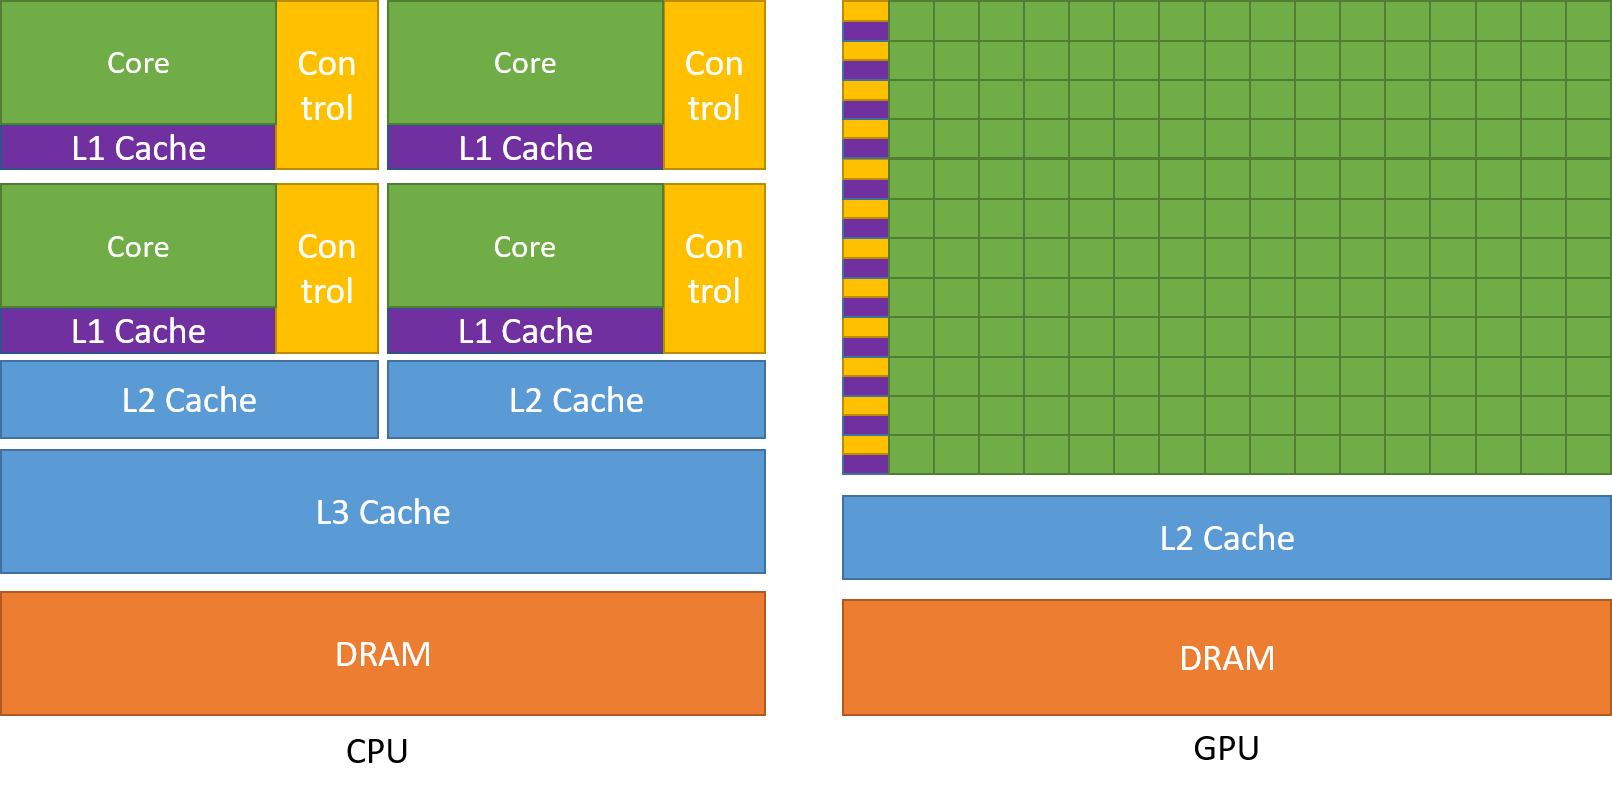
\includegraphics[width=0.9\linewidth]{images/cpu_vs_gpu.png}
\end{bonus}

\begin{defi}{Field Programmable Gate Array (FPGA)}
    % TODO: https://de.wikipedia.org/wiki/Field_Programmable_Gate_Array (Quelle)
    Ein \emph{FPGA} (Akronym für \emph{Field Programmable Gate Array}) ist ein integrierter Schaltkreis (IC) der Digitaltechnik, in welchen eine logische Schaltung geladen werden kann.

    Anders als bei der Programmierung von Computern, Mikrocontrollern oder Steuerungen bezieht sich hier der Begriff Programmierung nicht nur auf die Vorgabe zeitlicher Abläufe, sondern vor allem auch auf die Definition der gewünschten Schaltungsstruktur.
    Diese wird mittels einer Hardwarebeschreibungssprache formuliert und von einer Erzeugersoftware in eine Konfigurationsdatei übersetzt, welche vorgibt, wie die physischen Elemente im FPGA verschaltet werden sollen.
    Man spricht daher auch von der Konfiguration des FPGA.
    Ohne diese hat der Baustein keine Funktion.
\end{defi}

\begin{bonus}[Field Programmable Gate Array]{Anwendung}
    Durch Konfiguration der intern vorhandenen Elemente können in einem \emph{FPGA} verschiedene Schaltungen und Funktionen realisiert werden.
    Diese reichen von Schaltungen geringer Komplexität, wie z. B. ein einfacher Synchronzähler oder Interfaces für Digitalbausteine, bis hin zu hochkomplexen Schaltungen wie Speicher-Controller und vollständige Mikroprozessoren.

    FPGAs werden in allen Bereichen der Digitaltechnik eingesetzt, vor allem aber dort, wo es auf schnelle Signalverarbeitung und flexible Änderung der Schaltung ankommt, um beispielsweise nachträgliche Verbesserungen an den implementierten Funktionen vornehmen zu können, ohne dabei direkt die Hardware ändern zu müssen.

    Ein großes Anwendungsgebiet ist die Erstellung von Prototypen in der ASIC-Entwicklung (\enquote{Application-Specific Integrated Circuit}), zum vorherigen Test sowie auch der Bereich Maintenance, in dem es darum geht, Elektroniken für alte, nicht mehr lieferbare digitale Bausteine oder Microcontroller vorzuhalten.

    Mit der Einführung der FPGAs wurden kompakte, anwenderspezifische Schaltungen in geringen Stückzahlen ermöglicht.
\end{bonus}